\documentclass{beamer}
\setbeamertemplate{navigation symbols}{}

\usepackage{beamerthemeshadow}
\usepackage{amsmath}
\usepackage{bm}

\begin{document}
\title{Information bounds and attractor dynamics of an associative memory trained via spike-timing dependent plasticity}  
\author{Clayton Seitz}
\date{\today} 

\begin{frame}[plain]
\titlepage
\end{frame}

\section{Introduction} 

\begin{frame}[plain]
\frametitle{Introduction} 

\end{frame}

\begin{frame}[plain]
\frametitle{RNNs trained with Hebbian learning rules}

\begin{center}
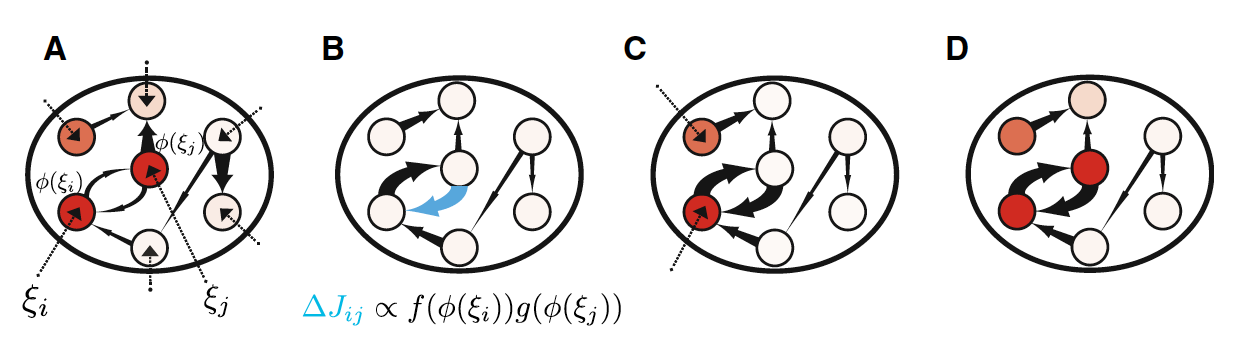
\includegraphics[scale=0.5]{network-diagram}
\end{center}

Let $W_{ij}$ be a matrix of recurrent weights that evolves when stimulated by 

\begin{equation*}
\xi(\bm{\mu}, \bm{\Sigma}) = \frac{1}{(2\pi)^{n/2}|\bm{\Sigma}|^{1/2}}\exp-\frac{1}{2}(\bm{r}-\bm{\mu})^{T}\bm{\Sigma}^{-1}(\bm{r}-\bm{\mu})
\end{equation*}

\footnote{\cite{peirera}}

\end{frame}
\begin{frame}[plain]
\frametitle{Inferring learning rules from firing rate distributions in ITC}

\begin{center}
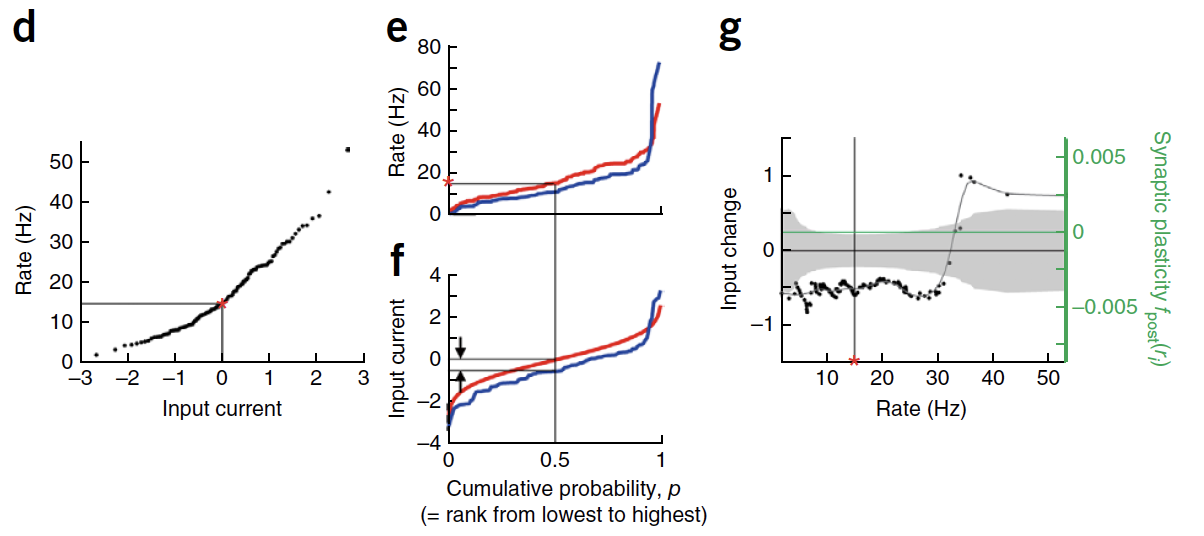
\includegraphics[scale=0.5]{learning-rules}
\end{center}

Inferring $\Delta W_{ij}$ from ITC neurons after presentation of novel and familiar images
\footnote{\cite{lim}}

\end{frame}

\begin{frame}[plain]
\frametitle{Inferring the transfer function from ITC data}

\vspace{0.2in}
All you can really observe is the firing rate distribution. Assume the input currents are Gaussian 

\begin{center}
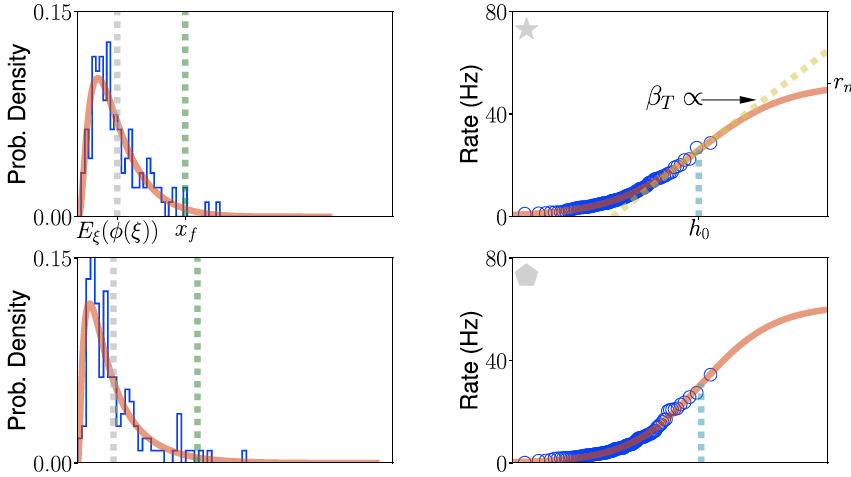
\includegraphics[scale=0.45]{transfer-function}
\end{center}

\footnote{\cite{peirera}}
\end{frame}

\begin{frame}[plain]
\frametitle{Presenting novel and familiar stimuli to the network}

\vspace{0.2in}

\begin{center}
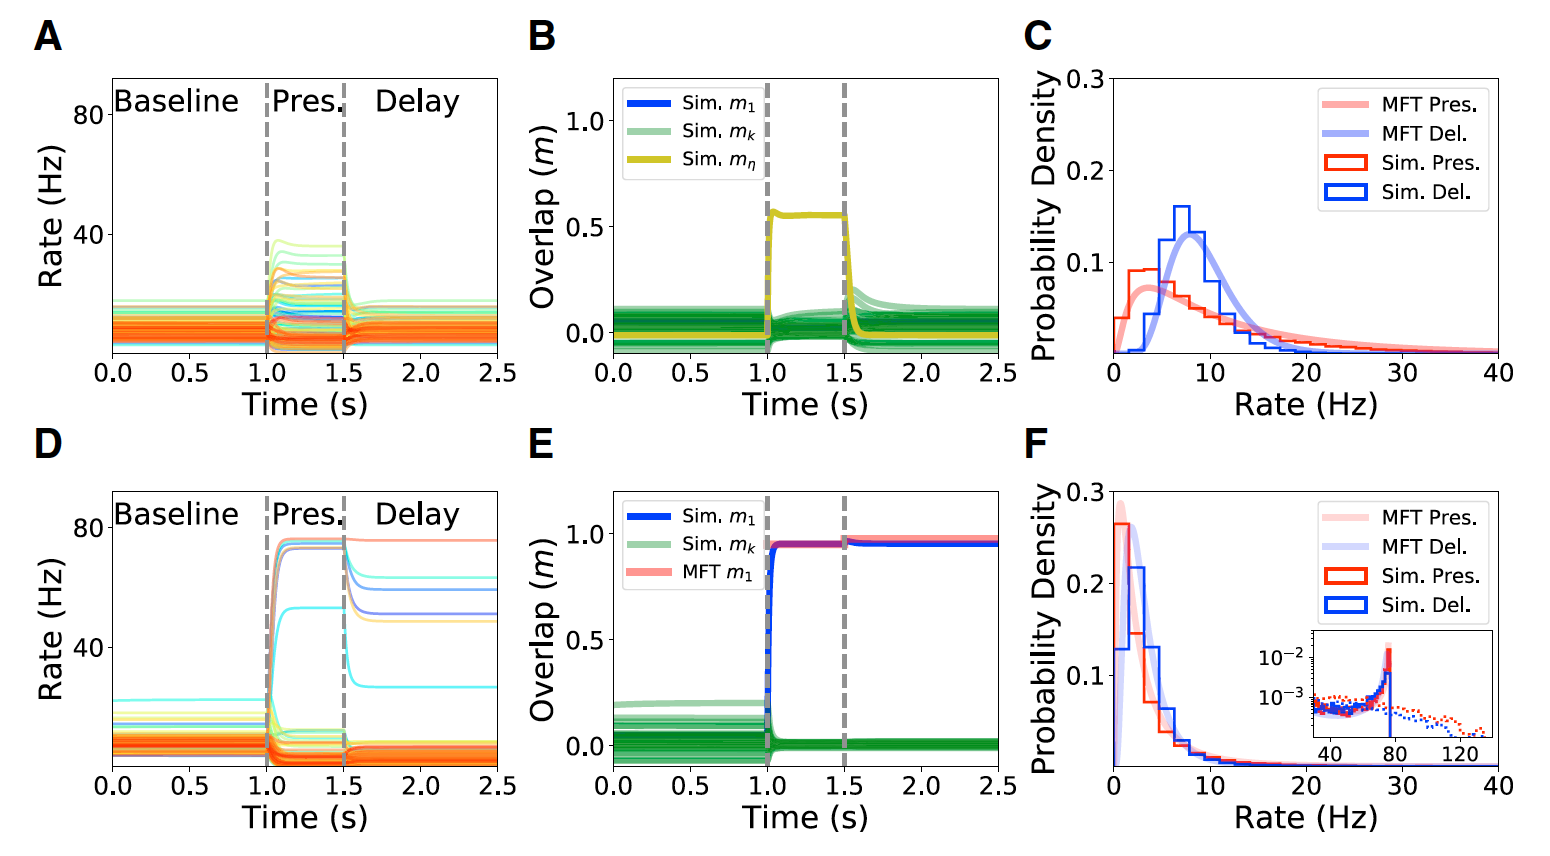
\includegraphics[scale=0.4]{novel-familiar}
\end{center}

\footnote{\cite{peirera}}

\end{frame}

\begin{frame}[plain]
\frametitle{Inferring learning rules from firing rate distributions in ITC}

Let the synaptic update be a separable function of the presynaptic $(\xi_{i})$ and postsynaptic $(\xi_{j})$ firing rates

\begin{equation*}
\Delta W_{ij} = f(\phi(\xi_{i}))g(\phi(\xi_{j}))
\end{equation*}

Evolution of the firing rate for neuron $i$ is

\begin{equation*}
\tau \dot{r_{i}} = -r_{i} + \phi(I + \sum_{j\neq i} W_{ij}r_{j})
\end{equation*}

Synaptic weight updates are weighted according to 

\begin{equation*}
W_{ij} = C_{ij}\sum  f(\phi(\xi_{i}))g(\phi(\xi_{j}))
\end{equation*}




\footnote{\cite{hopfield}}
\end{frame}

\begin{frame}[plain]
\frametitle{A recurrent firing-rate model}

The total input current $I$ to a neuron with $n$ inputs is given by

\begin{equation*}
r = F(\sum_{n} w_{n} \int_{-\infty}^{t}d\tau K(t-\tau)u(\tau))
\end{equation*}

where $K = \frac{1}{\tau}\exp(-t/\tau)$. Say we have a white-noise input $\bm{x}$. The rate-vector $\bm{v}$ evolves according to

\begin{equation*}
\tau \frac{d\bm{v}}{dt} = F(\bm{x} + \bm{M}\cdot \bm{z}) - \bm{z}
\end{equation*}


\end{frame}


\begin{frame}[plain]
\frametitle{Relating branching to firing rates} 


\begin{equation*}
\mathcal{L} = \alpha\sum_{t} (r(t) - \hat{r})^{2}
\end{equation*}

\begin{center}
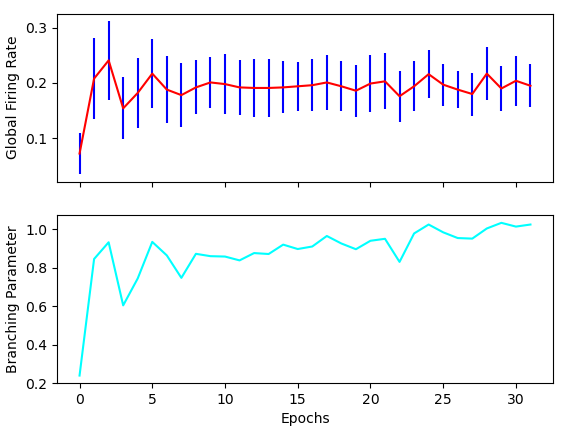
\includegraphics[scale=0.5]{alpha-1ms-bin}
\end{center}

\begin{equation*}
p_{ee} = 0.16 \; p_{ie} = 0.318 \;  p_{ei} = 0.244 \; p_{ii} = 0.343
\end{equation*}

\end{frame}

\begin{frame}[plain]
\frametitle{Relating branching to firing rates}  

\begin{equation*}
\mathcal{L} = \alpha\sum_{t} (r(t) - \hat{r})^{2}
\end{equation*}

\begin{center}
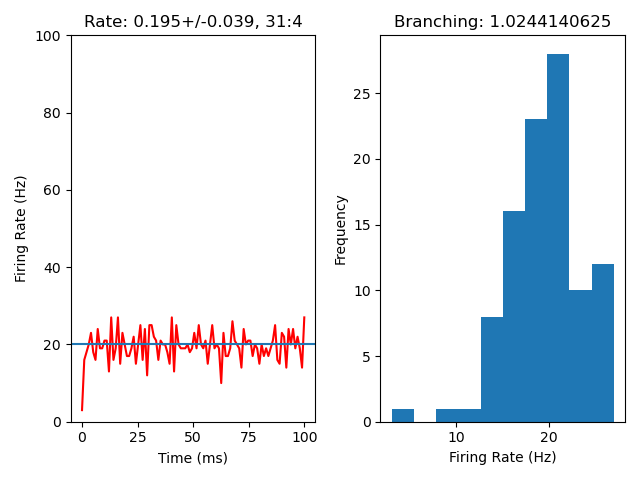
\includegraphics[scale=0.5]{last-epoch}
\end{center}


\end{frame}

\begin{frame}[plain]
\frametitle{} 

But optimization of $\mathcal{L}$ shows a sparse response

\begin{center}
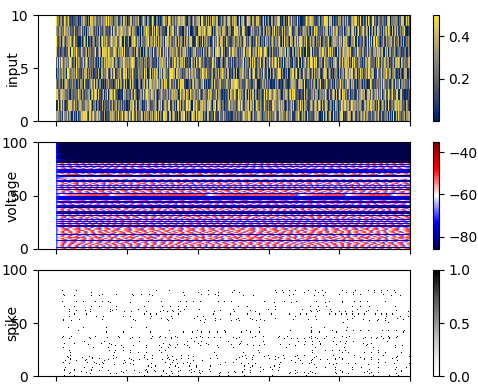
\includegraphics[scale=0.7]{alpha-traces}
\end{center}

\end{frame}


\begin{frame}[plain]
\frametitle{Balancing excitation and inhibition} 
The above analysis says nothing about excitatory and inhibitory subpopulations. How can you get critical dynamics in this case?

\end{frame}


\begin{frame}[plain]
\frametitle{Balancing internal and recurrent inputs} 

We know something about the balance of excitation and inhibition that gives critical dynamics. What about the balance between input and recurrence? (Cramer et al. 2020)


\begin{center}
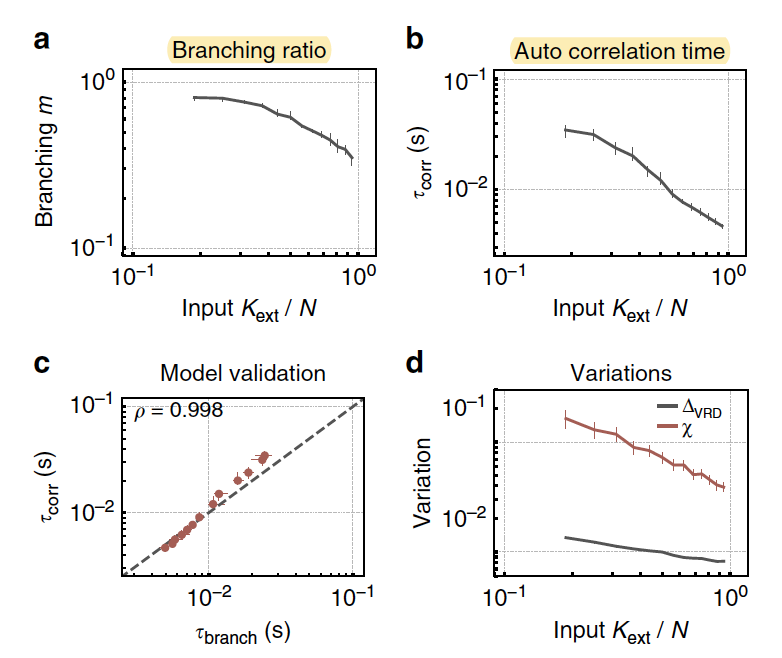
\includegraphics[scale=0.55]{cramer-criticality}
\end{center}

\end{frame}

\begin{frame}[plain]
\frametitle{Balancing internal and recurrent inputs} 
\end{frame}


\begin{frame}[plain]
\frametitle{Higher order correlations} 

Does the correlation structure of the network depend on the correlation structure of the stimulus?

\begin{center}
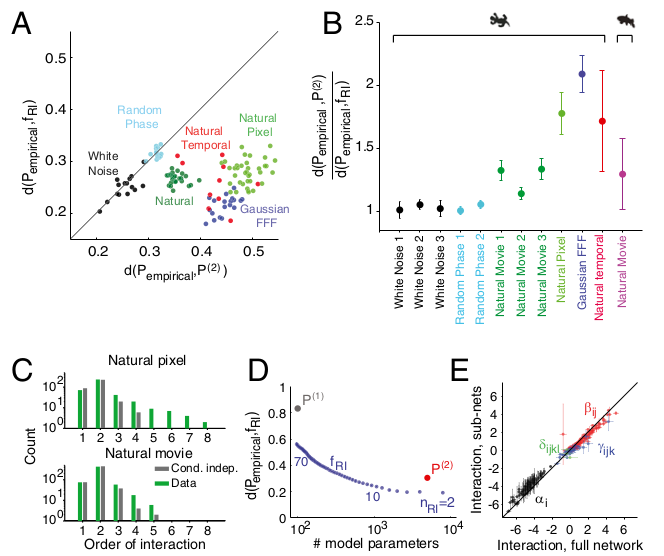
\includegraphics[scale=0.35]{higher-order-interactions}
\end{center}

\end{frame}


\begin{frame}[plain]
\frametitle{RNN Gradients} 

Say we have a model $\Phi = (W^{0},W^{1})$ and want to use gradient descent to train a network to have a target rate or a target branching parameter. The rate and its associated loss for a single unit is

\begin{equation*}
r(t) = \frac{1}{\Delta t}\int_{t}^{t+\Delta t} d\tau \langle \rho(\tau)\rangle\;\;\;\;\;\mathcal{L} = \alpha(r-r_{0})^{2}
\end{equation*}

We would like the standard update 

\begin{equation*}
\Delta W_{ij} = -\eta \frac{\partial\mathcal{L}}{\partial W_{ij}}
\end{equation*}


But it is intractable to compute $\frac{\partial\mathcal{L}}{\partial W_{ij}}$ since $\rho(t)$ depends on other neurons through space and time.


\end{frame}


\begin{frame}[plain]
\frametitle{Factorizing loss gradients for BPTT} 

BPTT involves unrolling an RNN into a large feedforward network where each layer is a time step. 

\begin{equation*}
\frac{\partial\mathcal{L}}{\partial W^{t}_{ij}} = \frac{\partial\mathcal{L}}{\partial h^{t}_{j}}  \frac{\partial h^{t}_{j}}{{\partial W^{t}_{ij}}} 
\end{equation*}

and the total gradient is a sum over the layers (time)

\begin{equation*}
\frac{\partial\mathcal{L}}{\partial W^{t}_{ij}} = \sum_{t} \frac{\partial\mathcal{L}}{\partial h^{t}_{j}}  \frac{\partial h^{t}_{j}}{{\partial W^{t}_{ij}}} 
\end{equation*}

\end{frame}

\begin{frame}[plain]
\frametitle{Deriving e-prop from BPTT} 

Consider the first term above. The hidden state is computed by some function $h_{j}^{t} = F(z_{j}^{t},h_{j}^{t-1} ,W)$. Backpropagating through time is then

\begin{equation*}
\frac{\partial\mathcal{L}}{\partial h^{t}_{j}} = \frac{\partial\mathcal{L}}{\partial z^{t}_{j}} \frac{\partial z^{t}_{j}}{\partial h^{t}_{j}}  + \frac{\partial\mathcal{L}}{\partial h^{t+1}_{j}} \frac{\partial h^{t+1}_{j}}{\partial h^{t}_{j}} 
\end{equation*}

which must be expressed recursively 

\begin{align*}
\frac{\partial\mathcal{L}}{\partial h^{t}_{j}} &= \frac{\partial\mathcal{L}}{\partial z^{t}_{j}} \frac{\partial z^{t}_{j}}{\partial h^{t}_{j}}  +  \left(\frac{\partial\mathcal{L}}{\partial z^{t+1}_{j}} \frac{\partial z^{t+1}_{j}}{\partial h^{t+1}_{j}}  + (...) \frac{\partial h^{t+2}_{j}}{\partial h^{t+1}_{j}} \right) \frac{\partial h^{t+1}_{j}}{\partial h^{t}_{j}} \\
&= L_{j}^{t} \frac{\partial z^{t}_{j}}{\partial h^{t}_{j}}  +  \left(L_{j}^{t+1} \frac{\partial z^{t+1}_{j}}{\partial h^{t+1}_{j}}  + (...) \frac{\partial h^{t+2}_{j}}{\partial h^{t+1}_{j}} \right) \frac{\partial h^{t+1}_{j}}{\partial h^{t}_{j}}\\
&= L_{j}^{t} \frac{\partial z^{t}_{j}}{\partial h^{t}_{j}}  +  \left(L_{j}^{t+1} \frac{\partial z^{t+1}_{j}}{\partial h^{t+1}_{j}}  + (...) \frac{\partial h^{t+2}_{j}}{\partial h^{t+1}_{j}} \right) \frac{\partial h^{t+1}_{j}}{\partial h^{t}_{j}}
\end{align*}

\end{frame}

\begin{frame}[plain]
\frametitle{Deriving e-prop from BPTT} 

Plugging into the original factorization gives

\begin{equation*}
\frac{\partial\mathcal{L}}{\partial W_{ij}} = \left(\sum_{t}L_{j}^{t} \frac{\partial z^{t}_{j}}{\partial h^{t}_{j}}  +  \left(L_{j}^{t+1} \frac{\partial z^{t+1}_{j}}{\partial h^{t+1}_{j}}  + (...) \frac{\partial h^{t+2}_{j}}{\partial h^{t+1}_{j}} \right) \frac{\partial h^{t+1}_{j}}{\partial h^{t}_{j}} \right)\frac{\partial h^{t'}_{j}}{{\partial W_{ij}}} 
\end{equation*}

You can then collect terms that are multiplied $L_{j}^{t}$

\begin{align*}
\frac{\partial\mathcal{L}}{\partial W_{ij}} &= \sum_{t}L_{j}^{t}\frac{\partial z^{t}_{j}}{\partial h^{t}_{j}} \left( \sum_{t'\leq t} \left(\prod_{t'} \frac{\partial h^{t'+1}_{j}}{\partial h^{t'}_{j}} \right)\frac{\partial h^{t'}_{j}}{{\partial W_{ij}}} \right) \\
&= \sum_{t}L_{j}^{t} \frac{\partial z^{t}_{j}}{\partial h^{t}_{j}}\mathbf{\epsilon_{ij}^{t}} = \sum_{t}L_{j}^{t} e_{ij}^{t} \\
\end{align*}

\end{frame}
\begin{frame}[plain]
\frametitle{Constraining the global firing rate distribution} 

We can define a constraint on the variance of the global firing rate (which simultaneously constrains the mean)

\begin{equation*}
\mathcal{L} = \beta(\sigma- \sigma_{r})^{2}
\;\;\;\;\;\;\; \sigma = \frac{1}{T}\sum_{t} (r - \mu_{r})^{2}
\end{equation*}

where we constrain branching by constraining the variance $s$ of the global firing rate where branching $\rightarrow 1$ as $s \rightarrow 0$.  

\begin{align*}
L_{j}^{t} = \frac{\partial \mathcal{L}}{\partial z_{j}^{t}} = \frac{\partial \mathcal{L}}{\partial \sigma}\frac{\partial \sigma}{\partial n} \frac{\partial n}{\partial z_{j}^{t}}
&= \pm \beta (\sigma- \sigma_{r}) \cdot (r-\mu_{r}) 
\end{align*}

Think push-pull. Some variation is necessary for refractoriness.

\end{frame}


\begin{frame}[plain]
\frametitle{Relating branching to firing rates and information} 

We have an ensemble of neurons with firing rates $\bm{r} = (r_{1}, r_{2} ..., r_{K})$

\begin{equation*}
\langle N \rangle = \sum_{k} r_{k}^{t}\Delta t = K  \Delta t \langle r \rangle
\end{equation*}

and we would like $\langle N \rangle$ to be constant. We draw a rate-vector from the joint distribution $\bm{r} \sim R(\bm{\mu}, \bm{\Sigma}$) 

\begin{equation*}
H(R) = H(P(r_{1}, r_{2}, ... r_{k})) \leq H\left(\prod_{k} P(r_{k})\right)
\end{equation*}

the upper bound maximizes mutual information at low noise

\begin{equation*}
I(X;R) = H(R) - H(R|X)
\end{equation*}

\end{frame}


\begin{thebibliography}{99} 
\bibitem[Peirera and Brunel, Neuron. 2018]{peirera}
\bibitem[Lim et al., Nature Neuroscience. 2015]{lim}
\bibitem[J.J. Hopfield PNAS. 1982]{hopfield}
\end{thebibliography}






\end{document}